

\documentclass{article}

% Recommended, but optional, packages for figures and better typesetting:
\usepackage{microtype}
\usepackage{graphicx}
\graphicspath{ {./} }
\usepackage{subfigure}
\usepackage{booktabs} % for professional tables
\usepackage{amsmath}

% hyperref makes hyperlinks in the resulting PDF.
% If your build breaks (sometimes temporarily if a hyperlink spans a page)
% please comment out the following usepackage line and replace
% \usepackage{icml2019} with \usepackage[nohyperref]{icml2019} above.
\usepackage{hyperref}

% Attempt to make hyperref and algorithmic work together better:
\newcommand{\theHalgorithm}{\arabic{algorithm}}

% Use the following line for the initial blind version submitted for review:
%\usepackage{icml2020}

% If accepted, instead use the following line for the camera-ready submission:
\usepackage[accepted]{icml2020}

% The \icmltitle you define below is probably too long as a header.
% Therefore, a short form for the running title is supplied here:
\icmltitlerunning{Text-to-image Implementation of Style GAN}

\begin{document}

\twocolumn[
\icmltitle{Text-to-image Implementation with Style-based Attentional GAN}

% It is OKAY to include author information, even for blind
% submissions: the style file will automatically remove it for you
% unless you've provided the [accepted] option to the icml2019
% package.

% List of affiliations: The first argument should be a (short)
% identifier you will use later to specify author affiliations
% Academic affiliations should list Department, University, City, Region, Country
% Industry affiliations should list Company, City, Region, Country

% You can specify symbols, otherwise they are numbered in order.
% Ideally, you should not use this facility. Affiliations will be numbered
% in order of appearance and this is the preferred way.
\icmlsetsymbol{equal}{*}

\begin{icmlauthorlist}
\icmlauthor{Fei Zheng fz2277}{equal,to}
\icmlauthor{Chirong Zhang cz2533}{equal,to}
\icmlauthor{Xiaoxi Zhao xz2740}{equal,to}
\end{icmlauthorlist}

\icmlaffiliation{to}{Department of Statistics, Columbia University, New York, USA}

% \icmlcorrespondingauthor{}{}

% You may provide any keywords that you
% find helpful for describing your paper; these are used to populate
% the "keywords" metadata in the PDF but will not be shown in the document
\icmlkeywords{Machine Learning, ICML}

\vskip 0.3in
]

% this must go after the closing bracket ] following \twocolumn[ ...

% This command actually creates the footnote in the first column
% listing the affiliations and the copyright notice.
% The command takes one argument, which is text to display at the start of the footnote.
% The \icmlEqualContribution command is standard text for equal contribution.
% Remove it (just {}) if you do not need this facility.


\printAffiliationsAndNotice{}  % leave blank if no need to mention equal contribution
% \printAffiliationsAndNotice{\icmlEqualContribution} % otherwise use the standard text.

\begin{abstract}
In this project, we propose a Style-Based Attentional Generative Adversarial Network (SBA-GAN) that allows unsupervised disentanglement of high-level attributes and an attention-driven refinement for text-to-image generation. Borrowing from StyleGan literature and AttnGan structure, this new generator can synthesize details at different regions of image by paying attentions to relevant parts in the text and by interpolating styles into different resolutions in the image. On CUB dataset, our generated 256*256 images have a higher inception score compared to existing methods. Detailed style and attention analysis is also performed by visualizing the different layers of SBA-GAN. 
\end{abstract}

\section{Introduction}

Text-to-image (T2I) generation is a an important machine learning task and an active research area in both computer vision and natural language processing. It is a fundamental problem in art generation, logo design, interior design and other computer-aided image synthesize. Recent years, significant progress has been made in text-to-image using generative adversarial networks \cite{gan}. 

In contrast to general image generation problems,
T2I generation is conditioned on texts instead of starting with random noise alone. Different T2I approaches have been made to generate more realistic and text-relevant images, such as in AttentionGAN \cite{attngan}, MirrorGAN \cite{mirrorgan}, ObjGAN \cite{objgan}, DMGAN \cite{dmgan}. However, due to entanglement caused by the input latent space which must follow the probability density of the
training data, it still remains challenging to generate high-resolution images align with the input text.

To address this issue, we propose a Style-Based Attentional Generative Adversarial Network (SBA-GAN). Motivated by the Style-Based Generator Architecture for Generative Adversarial Networks (GAN)\cite{stylegan}, which implemented style transfer techniques\cite{styletransferog} in the generative network. The overall architecture of the SBA-GAN
is illustrated in Figure \ref{model}. The two main parts of SBA-GAN is BERT (text encoder) and an attentional style generator. Unlike previous networks which pervasively utilize recurrent neural network (RNN)\cite{lstm} as the text encoder, we proposes to use the pre-trained BERT \cite{bert}. The other new component is the attentional style generator which adopts the general architecture of AttnGAN\cite{attngan} and incorporate the style module described in \cite{stylegan}.

To generate a single image, our generator starts from a learned constant input instead of a latent random variable and it takes the sentence-level and word-level vectors features to put "constraints" on the generated images. The conditional loss is calculated to guarantee that the text and image are aligned. Our generator also adjusts the “style” of the image at each convolution layer based on the latent
code, which can directly control the strength of image features at different scales. Our code is available at \href{https://github.com/zhengfei0908/SBA-GAN}{https://github.com/zhengfei0908/SBA-GAN}.

We evaluate our methods using the same loss functions in AttnGAN\cite{attngan} and calculate the inception score\cite{inception} of generated images. \footnote{The calculation of inception score in AttnGAN is the same with StackGAN which uses the deprecated tensorflow1 and the corresponding inception model, we found another way to calculate the inception score which might be different from the AttnGAN} Our inception score on CUB dataset \cite{WahCUB_200_2011} is slightly higher than the existing results.

\section{Related work}

Based on the DCGAN\cite{dcgan}, Reed\yrcite{text2image} has proposed an architecture to do text-to-image translation. In his algorithm GAN-CLS\cite{text2image}, he introduces a third type of input consisting of real images with mismatched text in discriminator in addition to the real/fake inputs. This provides an additional signal to the generator. Also, he explores the disentangling of style and content by inverting the generator for style and it turns out captions alone are not informative for style prediction.

AttnGAN \cite{attngan} first came up with the idea to synthesize fine-grained details at different subregions of the image by paying attention to the relevant words in the natual language desciption. MirrorGAN\cite{mirrorgan} borrow the idea of circleGAN\cite{cyclegan} and generate image from text and text back from image.

With the appearance of StyleGAN\cite{stylegan}, researchers have proposed new network structure using it and have observed a great increse in FID score\cite{fid}. LOGAN \cite{logan} which proposes a conditional GAN structure with StyleGAN implemented, has successfully generate conditional logos with high FID. But the paper did not discuss the alignment between the image and the logo label and indeed, some generated logos do not seem to be properly generated conditioned on the given label. Our model, tries to address this problem and introduce the similarity measure between text and the generated images.


\begin{figure*}[ht]

\centering
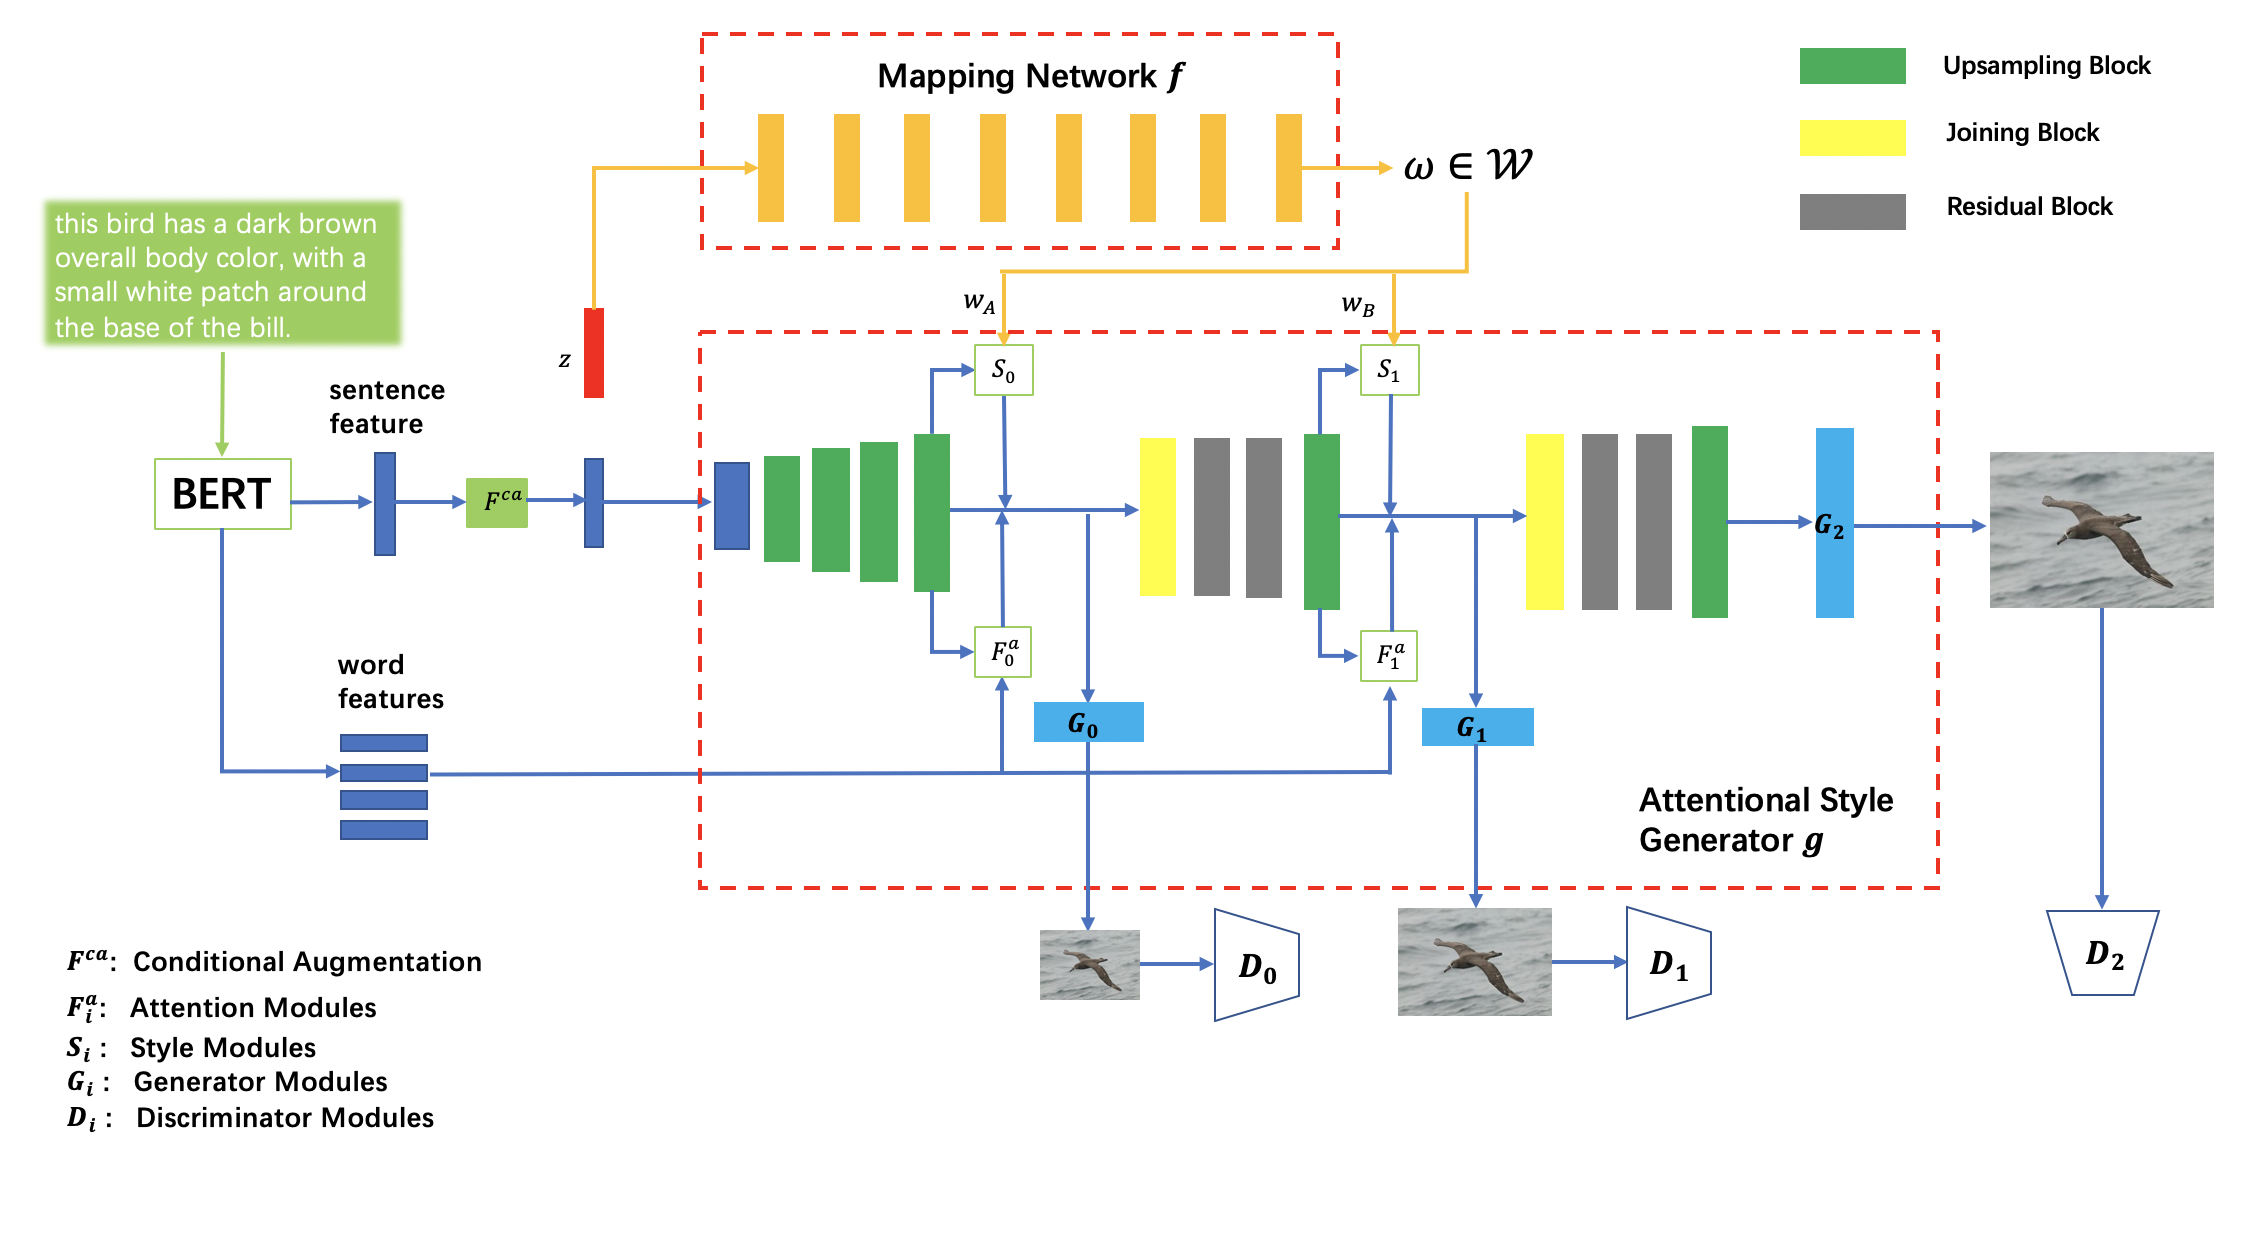
\includegraphics[width=450pt, height=220pt]{report/network.png} 
\caption{The architecture of proposed SBA-GAN. The figure is adapted mainly from AttnGAN\cite{attngan}. The mapping network $\math{f}$ maps latent variable $\math{z}$ to an intermediate latent space $\mathcal{W}$, as proposed in StyleGAN\cite{stylegan}. Attentional style generator $\math{g}$ generates images with different resolutions from a conditionally augmented sentence feature. During each step, style modules($S_0$ and $S_1$) and attention modules($F_0^a$ and $F_1^a$) inject style and word features information respectively.}
\label{model}
\end{figure*}

\section{Methods: Style-Based Attentional Generative Adversarial Network}
As shown in Figure \ref{model}, SBA-GAN integrates StyleGAN\cite{stylegan} and AttnGAN\cite{attngan}. Unlike common practice, we separates latent variable $\math{z}$ from conditional sentence feature vector and use disentangled latent variable $\math{w}$ to control the style of images through the style module(AdaIN) during generation process. Technically, SBA-GAN can be divided into two main parts: text encoder and attentional style generator.


\subsection{Text Encoder}
First, we introduce the text encoder module that transforms the texts to features. We try two types of the text encoders, plain RNN with LSTM units\cite{lstm} and BERT\cite{bert}. LSTM helps to handle long term dependency problems which is now a standard method in natural language processing while BERT is a great breakthrough in the domain of pre-trained NLP. In previous work in text-to-image field like AttnGAN\cite{attngan} and MirrorGAN\cite{mirrorgan}, BERT is rarely applied to extract information from sentence. In our experiments, we compare the pre-trained BERT with our baseline, LSTM and BERT version outperforms the baseline. 
In terms of how the text encoders are used, we embed the given text description into both word-level features that work mainly in attention modules and sentence-level features that work mainly in generation process.

Due to the diversity of the text domain or language and in order to enhance the model robustness, we introduce some noises in sentence-level features by using Conditional Augmentation\cite{stackgan}. In Figure \ref{model}, we use $F^{ca}$ to represent this module.
\begin{equation}
    \bar{e}_{ca} = F^{ca}(\bar{e}),
\end{equation}
where $\bar{e} \in \mathcal{R}^{D}$, $\bar{e}_{ca} \in \mathcal{R}^{D'}$, $D$ is the dimension of embedding features and $D'$ is the dimension after augmentation.

Unlike common practice in conditional GAN, we only input the augmented sentence feature into next generator rather than concatenate it with random latent variable $\math{z}$.

\subsection{Attentional Style Generator}
Next we introduce the style-base attentional generator. We adopt the general architecture described in AttnGAN\cite{attngan} because of its outstanding results.

In the mapping network $\math{g}$, we use a 8-layer MLP to disentangle the latent variable $z$ into latent variable $w$. And as proposed in StyleGAN\cite{stylegan}, the mapping network consists of 8 fully connected layer without bias.
\begin{equation}
    w = MLP(z)
\end{equation}

In the generation part, we follow the practice of AttnGAN\cite{attngan} and use the structure of StackGAN\cite{stackgan} to generate images with resolution $64^2$, $128^2$ and $256^2$.

During each generation block, attention modules $F_i^a$ mixes word-level features $e \in \mathcal{R}^{D \times T}$ and image features $h \in \mathcal{R}^{\hat{D} \times T}$ from previous block and retrieves the most relevant word vectors for generating different sub-regions of the image. Word-level features first are converted into the common semantic space with same dimension as image features,
\begin{equation}
    e^{'} = Ue,
\end{equation}
where $U \in \mathcal{R}^{\hat{D} \times D}$. The result $F_i^a(e, h) \in \mathcal{R}^{\hat{D} \times N}$($N$ is the number of sub-regions) is feature vectors of sub-regions, which can be represented as $(c_0, c_1,..., c_{N-1})$. For the $j^{th}$ sub-region,
\begin{equation}
    c_j = \sum_{i=0}^{T-1} \beta_{j, i}e_i^{'}, \beta_{j,i} = \frac{e^{s_{j,i}^{'}}}{\sum_{k=0}^{T-1} e^{s_{j,k}^{'}}},
\end{equation}
where $s_{j,k}^{'} = h_j^T e_i^{'}$. $\beta_{j,i}$ indicates the attention weight of the $i^{th}$ word for the $j^{th}$ sub-region of the image.

Style modules inject style from disentangled latent space $\mathcal{W}$ to generation process. Following the practice as in StyleGAN\cite{stylegan}, we first use an affine transformation to specialize $\math{w}$ to \textit{style} $y \in \mathcal{R}^{2 \times \hat{D}}$, which can control the adaptive instance normalization(AdaIN) operation in each generation block.The AdaIN operation is defined as:
\begin{equation}
    AdaIN(x_i, y) = y_{s,i} \frac{x_i - \mu(x_i)}{\sigma(x_i)} + y_{b,i},
\end{equation}

where each feature map $x_i$ is normalized separately, and then scaled and biased using the corresponding scalar components from \textit{style} $y$. So the dimension of $y$ is twice the number of features on that layer.

Finally, we combine original image features, attentional image features and style injected image features to generate images at the next stage.

\subsection{Objective functions}
Following common practice in text-to-image field, we first employ the GAN loss that embodies both conditional and unconditional. During each stage of training process, we train the generator and discriminator alternatively. Specifically, the generator $G_i$ is trained to minimize the generator loss:
\begin{equation}
    \mathcal{L}_{G_i} = -\frac{1}{2}\mathrm{E}_{\hat{x} \sim P_{G_i} [log(D_i(\hat{x})]} - \frac{1}{2}\mathrm{E}_{\hat{x} \sim P_{G_i} [log(D_i(\hat{x}, \bar{e})]}
\end{equation}

And the discriminator $D_i$ is trained to minimize the discriminator loss:
\begin{align}
    \mathcal{L}_{D_i} = &-\frac{1}{2}\mathrm{E}_{x \sim P_{data} [log(D_i(x)]} - \frac{1}{2}\mathrm{E}_{\hat{x} \sim P_{G_i} [log(1 - D_i(\hat{x})]} \nonumber \\
    &- \frac{1}{2} \mathrm{E}_{x \sim P_{data} [log(D_i(x, \bar{e})]} - \frac{1}{2}\mathrm{E}_{\hat{x} \sim P_{G_i} [log(1 - D_i(\hat{x}, \bar{e})]},
\end{align}
where $x$ is from the true image distribution $P_{data}$ and $\hat{x}$ is from the model distribution $P_G$. The unconditional loss determines whether the image is real or fake and the conditional loss determines whether the image matches the sentence or not.

Apart from the common GAN loss, we also employ DAMSM loss\cite{attngan}. DAMSM is proposed in AttnGAN and achieved good results. We consider this loss for two reasons. One is that we regard this loss as the critical reason that AttnGAN can achieve such good results. The other is that we also need to pre-train our BERT. DAMSM can be used to train BERT individually, which is fit for our limited computation resource.

So the total generator loss and the discriminator loss can be defined as below:
\begin{equation}
    \mathcal{L}_{G} = \sum_{i=0}^{L-1} G_i + \lambda L_{DAMSM}
\end{equation}
\begin{equation}
    \mathcal{L}_{D} = \sum_{i=0}^{L-1} D_i
\end{equation}


\section{Results}
\begin{figure*}[htbp]

\centering
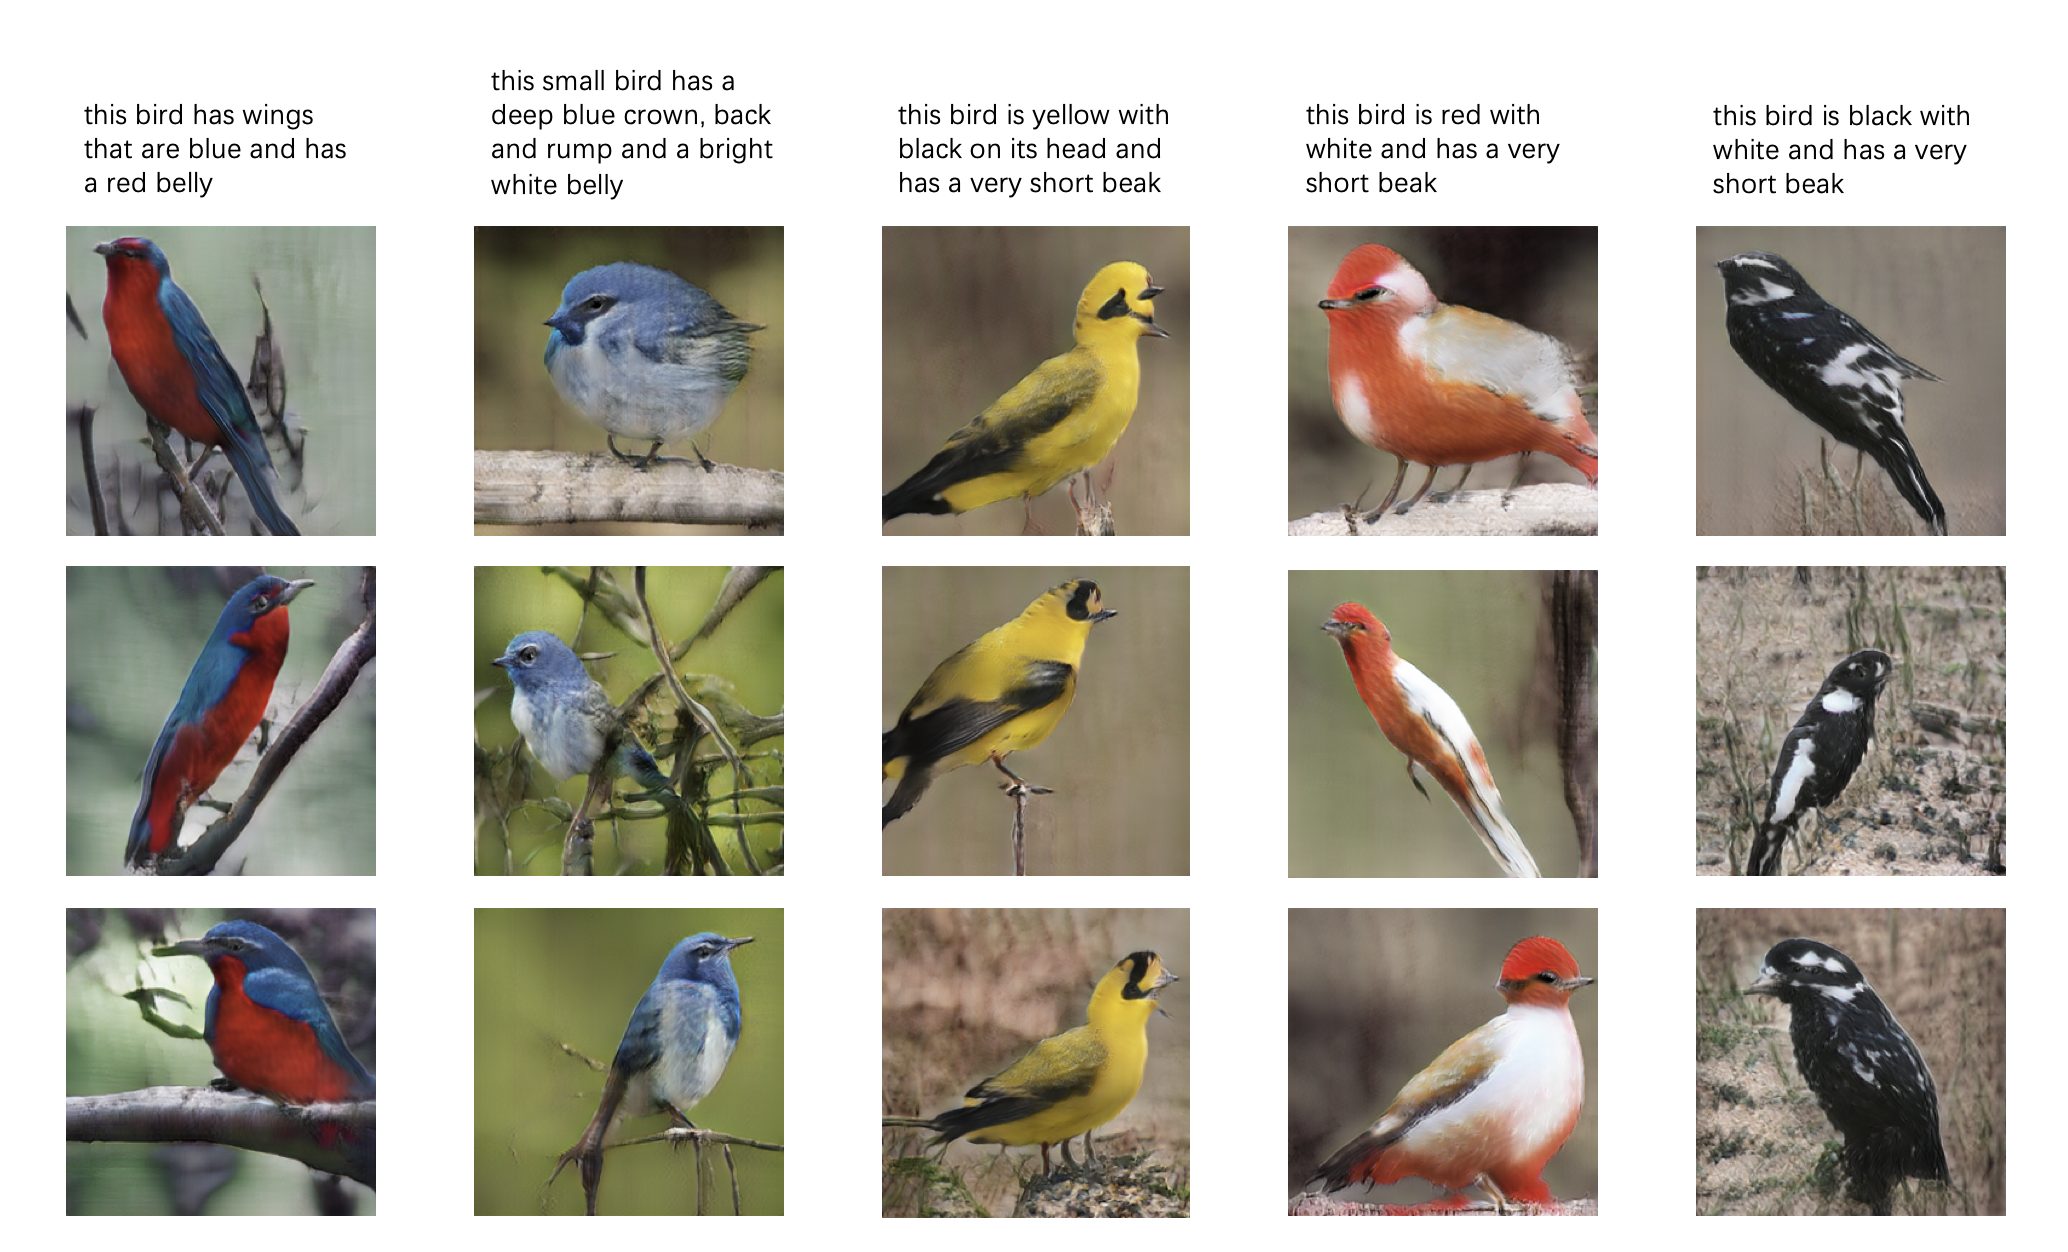
\includegraphics[width=450pt, height=250pt]{report/fig1.png} 
\caption{Examples of images generated by our best model(BERT with style) conditioned on
customized text descriptions. The vertical variate is from the different latent variable $z$.  }
\label{fig1}
\end{figure*}

Experimentation is carried out to evaluate the
proposed SBA-GAN. We compare our SBA-GAN result with previous state-of-the-art GAN models for text to image synthesis.

\subsection{Experiment Setup}
\subsubsection{Dataset}

Same as previous text-to-image methods\cite{attngan,mirrorgan}, our method is evaluated on CUB dataset.\cite{WahCUB_200_2011}

The CUB bird dataset contains 8,855 training images and 2,933
test images belonging to 200 categories, each bird image has 10 text description.

\subsubsection{Evaluation Criteria}

We will evaluate our approach by calculating the inception score\cite{inception} of generated images.

Inception score is a quantitative evaluation measure to the objectiveness and diversity of generated images but cannot reflect whether the generated image is well conditioned on the given text description. 

% R-precision is on the other hand, an evaluation metric to measure the similarity of images and the corresponding texts. We calculate the cosine similarities between the image feature and the text feature and count the average accuracy at the different settings: top-r. If the ground truth falls into the top-r candidates, then the image and text are considered aligned, otherwise not.



\subsubsection{Implementation Details}
For the text encoder part, we freeze most layers but the last layer of pre-trained BERT model \textit{bert-base-uncased}. The embedding dimensions for words features and sentence feature are both 256. The max sentence length is 20. For the image encoder part, we follow the practice of AttnGAN\cite{attngan} and use pre-trained InceptionV3\cite{inception2} to extract image features. Considering that we also use a pre-trained BERT in text encoder part, not a RNN model trained from scratch, we make the last three feature layers trainable. This proves to be a good practice. The image feature dimension is 256 and each image is divided into $17 \times 17$ sub-regions to calculate image-text matching score(\textit{i.e.}, DAMSM loss). Because of the limited computation source, we employ the same hyperparameters as AttnGAN\cite{attngan} for DAMSM module. The generator and discriminators are trained alternatively with learning rate 0.0002. For the baseline model(only adding styles), we train 600 epoches and for the latter models, we train only 200 epoches.

\subsection{Main Results}

We conduct four different models based on attention GAN(Baseline model) and compare them by inception score.
"+ style" is the baseline model combined with style($s_0$ and $s_1$ in Figure\ref{fig1}).
"+ BERT" replaces LSTM text encoder in "+ style"  with BERT text encoder.
In "+ Style mixing", $s_0$ and $s_1$ are generated from different $w$ and is trained on "+ BERT".

The result shows that both BERT and style module help to improve the results.

\begin{table}[h!]
\centering
\begin{tabular}{ | p{2cm} || p{1cm} | } 
\hline
Baseline & 4.36  \\ 
\hline
+ style & 5.05 \\ 
\hline
+ BERT & 5.12 \\ 
\hline
+ Style mixing & 4.75 \\ 
\hline
\end{tabular}
\caption{Inception score from different models}
\label{table:1}
\end{table}

\subsubsection{Generation Results}

Subjective visualization is presented in Figure \ref{fig2},\ref{fig3}. All the figures are generated from our "+BERT" model. 
It can be seen that the image details can be generated precisely by our model. i.e. text information can be presented in the figure. For example, in the first column, all three plots are able to present blue wings and red belly as described in the text as well as the short information in the third column.

Besides, the precision of our model can be shown in figure \ref{fig2} as well. Two sentences which only differ in color are used to generate two plots. In the first row, the bird has white belly, gray check patch and yellow crown while the bird in the second row has yellow belly, white check patch and gray crown instead.

\begin{figure}[htbp]

\centering
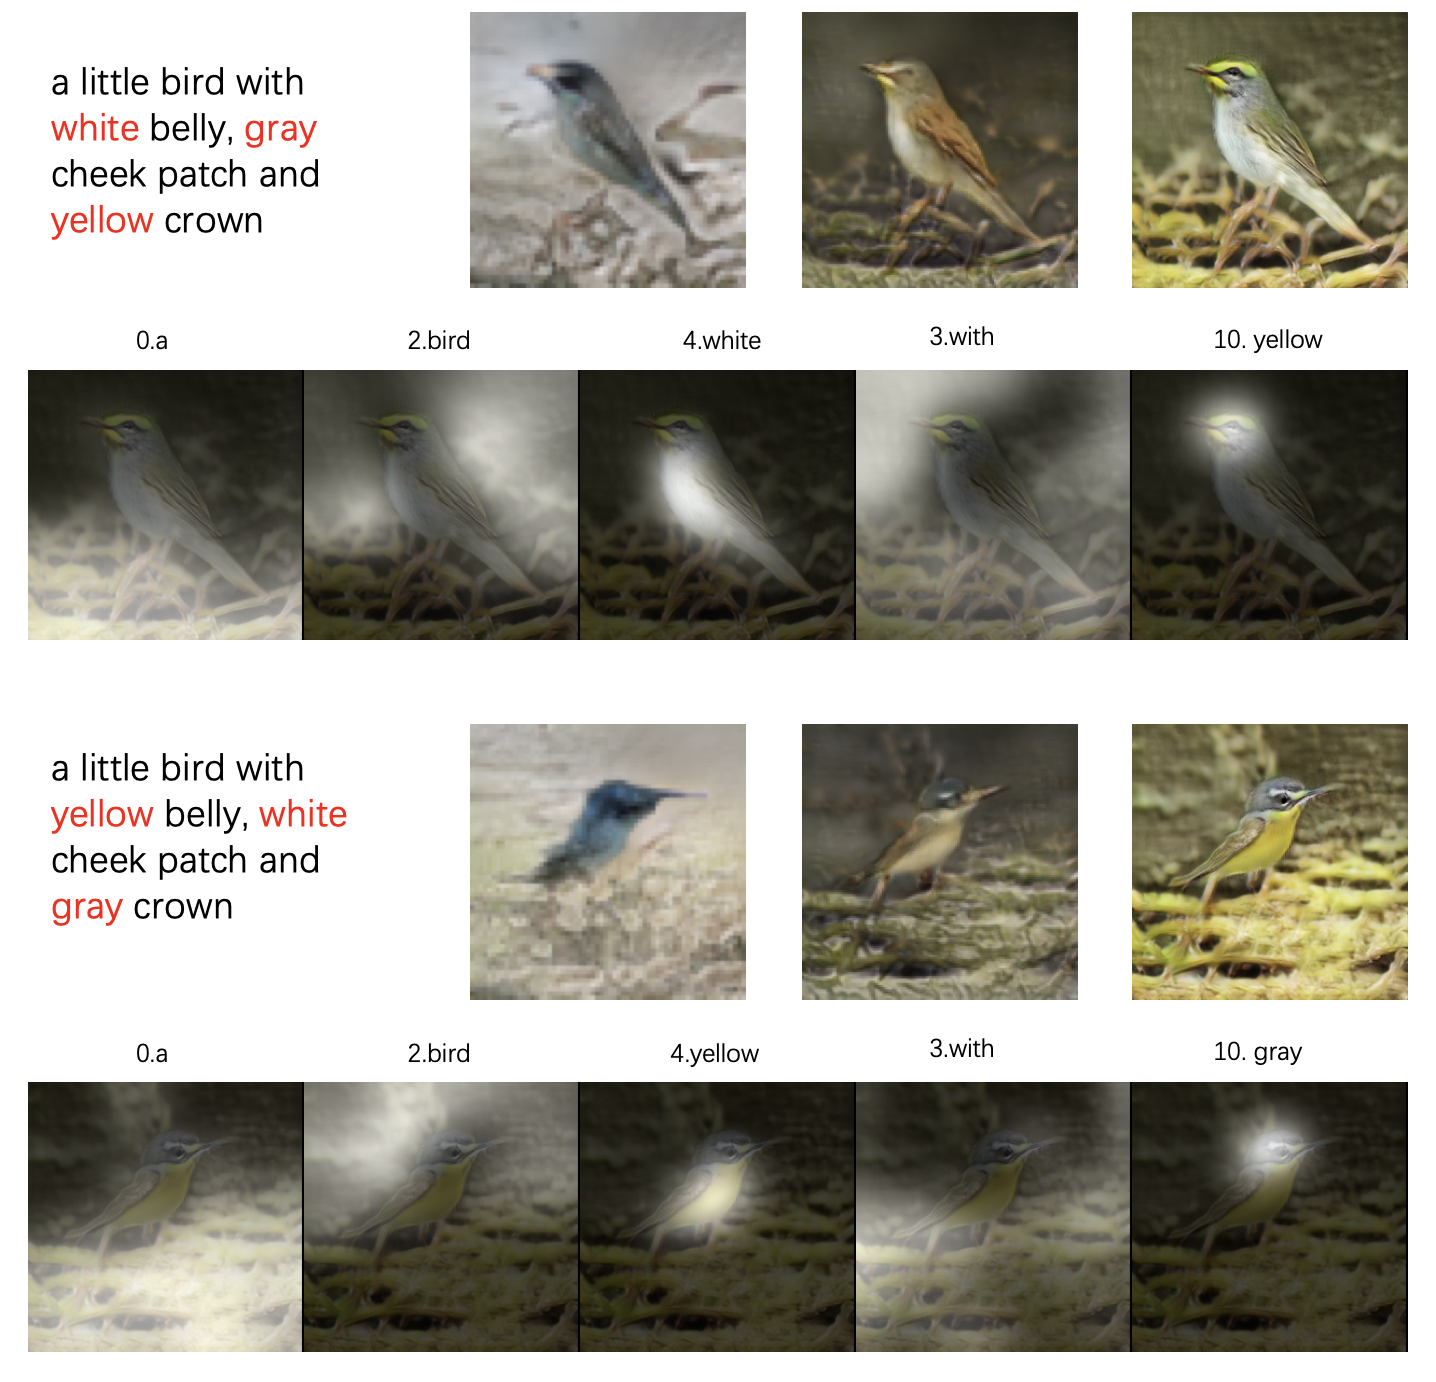
\includegraphics[width=250pt, height=200pt]{report/fig2.png} 
\caption{Examples of images generated by our best model(BERT with style) conditioned on
customized text descriptions. The vertical variate is from the different latent variable $z$.  }
\label{fig2}
\end{figure}


\subsubsection{Attention Analysis}

Attention visualization is presented in Figure\ref{fig2},\ref{fig3} which further proves that our model is able to learn how to generate the plot precisely.
Figure\ref{fig2} shows that attention can be allocated to correct positions. For example, attention of none-semantic words like "a", "bird","with" are allocated globally while attention of semantic words like "while" and "yellow" are allocated precisely on the right place.

Figure\ref{fig3} present how the model learn to generate plot. For example, the attention of word "green" in the stage one and stage two is different. In the first plot, the highlight part is approximated, a large area while in stage 2, it is located in the wings accurately. 


\begin{figure}
\centering
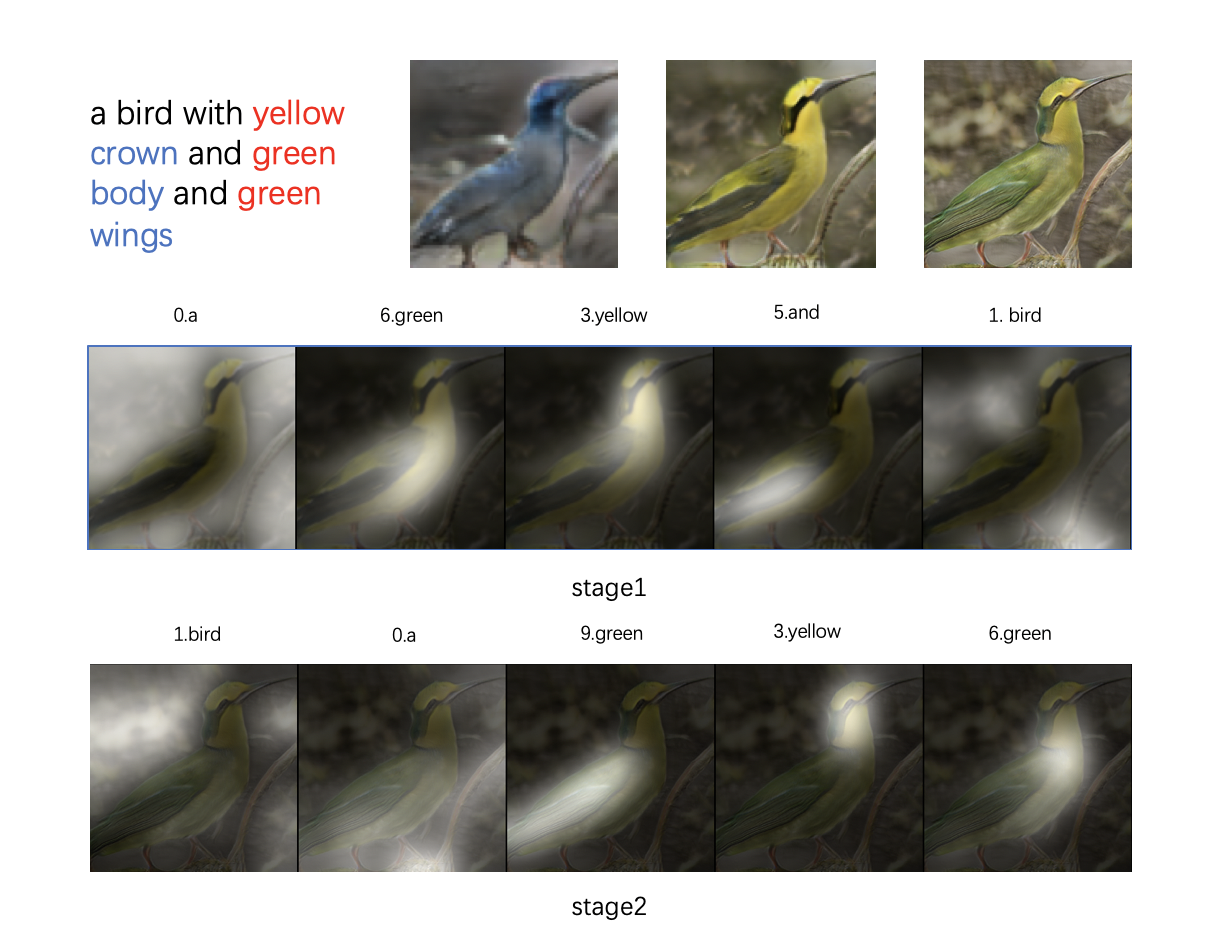
\includegraphics[width=250pt, height=200pt]{report/fig3.png} 
\caption{Examples of attention images generated by our best mode conditioned on customized text descriptions.   }
\label{fig3}
\end{figure}

\subsubsection{Style Mixing Analysis}
\begin{figure}
\centering
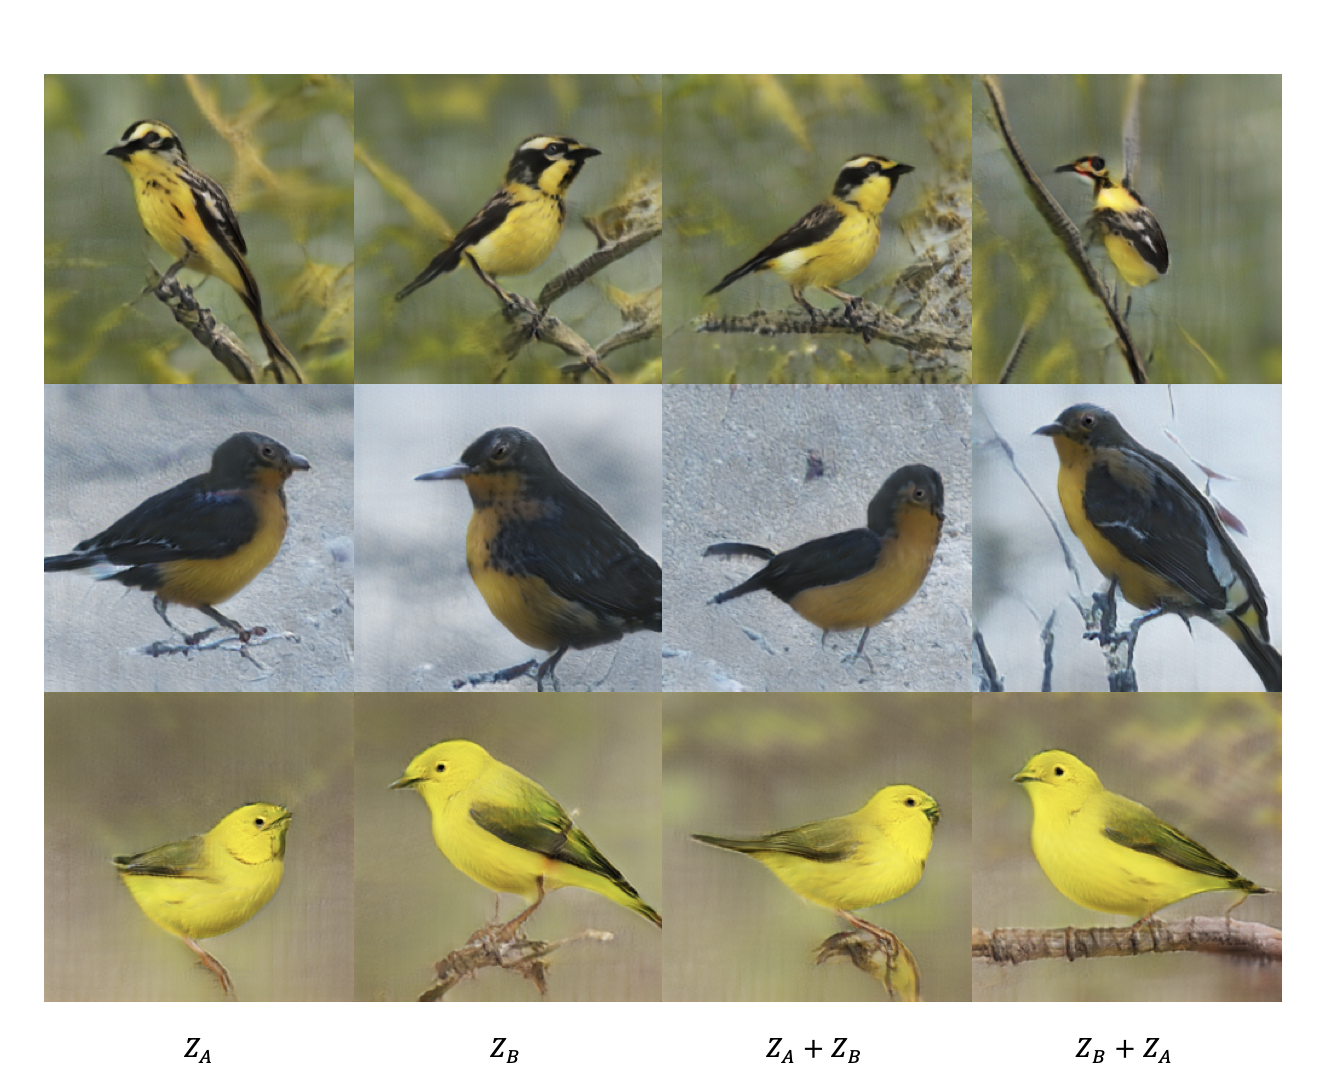
\includegraphics[width=250pt, height=200pt]{report/fig4.png} 
\caption{Examples of mixing style results. The first and the second column are generated by single random latent variable $Z_A$ and $Z_B$ respectively. The third column are generated by injecting $Z_A$ first and $Z_B$ second and the fourth column reverse.}
\label{fig4}
\end{figure}
As proposed in StyleGAN\cite{stylegan}, mixing regularization can encourage the styles to localize and we employ this strategy to make our generator more robust. To be specific, we generate two random latent variables $z_A$ and $z_B$, pass them through mapping network respectively and get $w_A$ and $w_B$. When generating an image, we should switch randomly from one to another with a certain probability. This technique prevents the network from assuming that styles are correlated.

For simplicity, we implement style mixing technique by injecting two different random latent variable in order without randomness. \ref{fig4} shows some styles mixing results. The pattern is not that significant but we can still detect a little. For example, the yellow bird on the third row and the third column has a long tail and a short beak, which is a combination of the original two birds. The worse inception score might be due to the training methods we use.


\section{Discussion}
\subsection{Conclusion}
In this project, we proposed a Style-based Attentinal GAN, named SBA-GAN, based on AttnGAN\cite{attngan} and StyleGAN\cite{stylegan}. We use BERT as our text encoder and employ adaptive instance normalization(\textit{i.e.},style injection) and style mixing technique. As a result, BERT encoder and adaptive instance normalization achieve inception score 5.05 and 5.12 respectively. Style mixing does not perform well as we thought first because of the computation resource and training strategy.

\subsection{Future Work}
 
We plan our future work in the following directions: experiments on larger datasets, more hyperparameter tuning, higher resolution images, more style mixing and change of the loss functions.

First, we only experiment our results on CUB birds dataset, but for most T2I tasks, COCO dataset \cite{coco} is also used for experiments. Due to our limited computational power and the huge image amount in COCO dataset, we choose not to do this experiment this time. However, to better compare our methods to existing networks, the experiment on COCO dataset is strongly helpful. Also, the text (condition) we are using now are mainly short sentences(less than 18 words), we can thus try some longer sentences with more detailed descriptions in the future. Since we are adopting the structure of StyleGAN, we can also try to implement a T2I on human faces dataset.

Second, we may want to perform more hyperparameter tuning in the future. We now freeze all the layers except the last pooling layer in BERT and we adopt all the hyperparameters used in AttnGAN instead of tuning our own parameters. If time and computation power permitted, we could search across the combination of hyperparameters, unfreeze more layers in BERT to get a better result.

Third, we start our image generation from 64*64 images and finish the generative process when we reach 256*256. We could start from 16*16 or even smaller images and incorporate more styles in our generative process. Also, we want to finish at images with higher resolution 512*512 or even 1024*1024 as StyleGAN does.

Last, we can try change our loss function to WGAN loss\cite{wgan} or add spectral normalization to our generator \cite{sagan}. We now can capture the color information in the text accurately but the shape, position of the birds can be wrong. Further some of the birds in our generated images do not look real (two heads, strange feet etc.). So we can try to change our loss function, alter the number of generator training between each discriminator and train for much longer periods.

\newpage

% In the unusual situation where you want a paper to appear in the
% references without citing it in the main text, use \nocite
\nocite{langley00}

\bibliography{example_paper}
\bibliographystyle{icml2020}


%%%%%%%%%%%%%%%%%%%%%%%%%%%%%%%%%%%%%%%%%%%%%%%%%%%%%%%%%%%%%%%%%%%%%%%%%%%%%%%
%%%%%%%%%%%%%%%%%%%%%%%%%%%%%%%%%%%%%%%%%%%%%%%%%%%%%%%%%%%%%%%%%%%%%%%%%%%%%%%
% DELETE THIS PART. DO NOT PLACE CONTENT AFTER THE REFERENCES!
%%%%%%%%%%%%%%%%%%%%%%%%%%%%%%%%%%%%%%%%%%%%%%%%%%%%%%%%%%%%%%%%%%%%%%%%%%%%%%%
%%%%%%%%%%%%%%%%%%%%%%%%%%%%%%%%%%%%%%%%%%%%%%%%%%%%%%%%%%%%%%%%%%%%%%%%%%%%%%%
% \appendix
% \section{Do \emph{not} have an appendix here}

% \textbf{\emph{Do not put content after the references.}}
% %
% Put anything that you might normally include after the references in a separate
% supplementary file.

% We recommend that you build supplementary material in a separate document.
% If you must create one PDF and cut it up, please be careful to use a tool that
% doesn't alter the margins, and that doesn't aggressively rewrite the PDF file.
% pdftk usually works fine. 

% \textbf{Please do not use Apple's preview to cut off supplementary material.} In
% previous years it has altered margins, and created headaches at the camera-ready
% stage. 
%%%%%%%%%%%%%%%%%%%%%%%%%%%%%%%%%%%%%%%%%%%%%%%%%%%%%%%%%%%%%%%%%%%%%%%%%%%%%%%
%%%%%%%%%%%%%%%%%%%%%%%%%%%%%%%%%%%%%%%%%%%%%%%%%%%%%%%%%%%%%%%%%%%%%%%%%%%%%%%


\end{document}


% This document was modified from the file originally made available by
% Pat Langley and Andrea Danyluk for ICML-2K. This version was created
% by Iain Murray in 2018, and modified by Alexandre Bouchard in
% 2019. Previous contributors include Dan Roy, Lise Getoor and Tobias
% Scheffer, which was slightly modified from the 2010 version by
% Thorsten Joachims & Johannes Fuernkranz, slightly modified from the
% 2009 version by Kiri Wagstaff and Sam Roweis's 2008 version, which is
% slightly modified from Prasad Tadepalli's 2007 version which is a
% lightly changed version of the previous year's version by Andrew
% Moore, which was in turn edited from those of Kristian Kersting and
% Codrina Lauth. Alex Smola contributed to the algorithmic style files.
